\documentclass[cover.tex]{subfiles}
\begin{document} \begin{refsection}


%%%%%%%%%%%%HEADING TITLE
\hfill\vspace{0.2cm}\begin{center}{\large \bfseries EXPERIMENT {\thesection}\par\Huge
 \import{\chapterpath/}{title}
 \\[5pt] \par}\vspace{0.2cm}\end{center}\par\noindent
 %%%%%%%%%%%%HEADING
 
 
\section*{Goal}
 \import{\chapterpath/}{goal}
\section*{Materials}
 \import{\chapterpath/}{materials}
\section*{Background}
\import{\chapterpath/}{background}
\section*{The experiment}
\import{\chapterpath/}{experiment}


%\import{\chapterpath/}{examplebox}
%%%%%BIBLIOGRAPHY
\printbibliography[heading=subbibliography]
%%%%%BIBLIOGRAPHY
%\section*{Lab Information}
% \begin{itemize}[label={$\blacksquare$}]
 %  \import{\chapterpath/}{labinfo}
% \end{itemize}
\section*{Procedure}
\import{\chapterpath/}{procedure}
%   \clearpage\mbox{}\clearpage






%%%%%%%%%%%%HEADING
\newgeometry{right=5cm}\thispagestyle{sidebar}\sidebar{   \vspace{1em}\vspace{1cm} \vfill \par\vspace*{1em}}\restoregeometry\clearpage \begin{multicols}{2}\begin{tcolorbox}[enhanced jigsaw,breakable,size=title,colback=mybrown!05,colframe=black,fonttitle=\bfseries,title=STUDENT INFO,pad at break=1mm, break at=15cm/0pt ]\vspace{0.2cm}\noindent Name:  \begin{Form}\TextField[name=NAME, width=4cm,height=0.5cm,multiline=false, borderstyle=U, bordercolor={black}]{} \end{Form}   \hspace{0.2cm}Date:  \begin{Form}\TextField[name=DATE, width=1.5cm,height=0.5cm,multiline=false, borderstyle=U, bordercolor={black}]{}\end{Form} \\\end{tcolorbox}\end{multicols}\hfill\vspace{0.2cm}\begin{center}{\large \bfseries Pre-lab Questions \par\Huge
\import{\chapterpath/}{title}
\\[5pt] \par}\vspace{0.2cm}\end{center}\par\noindent\uline{  \hfill \normalsize \hfill       }
%%%%%%%%%%%%HEADING
\import{\chapterpath/}{prelab}
%\clearpage\mbox{}\clearpage

 
 
 
 
 %%%%%%%%%%%%HEADING
\newgeometry{right=5cm}
\thispagestyle{sidebar}
\sidebar{%
  \vspace{1em}
  \vspace{1cm}
  \vfill
  \par\vspace*{1em}
}
\restoregeometry
\clearpage 
\begin{sidewaystable}[ph!]
\begin{multicols}{2}
\begin{tcolorbox}[enhanced jigsaw,breakable,size=title,
colback=mybrown!05,colframe=black,fonttitle=\bfseries,
title=STUDENT INFO,pad at break=1mm, break at=5cm/0pt ]
\vspace{0.2cm}
\noindent Name:  \begin{Form}\TextField[rotation=90,name=NAME, width=4cm,height=0.5cm,multiline=false, borderstyle=U, bordercolor={black}]{} \end{Form}   \hspace{0.2cm}Date:  \begin{Form}\TextField[rotation=90, name=DATE, width=1.5cm,height=0.5cm,multiline=false, borderstyle=U, bordercolor={black}]{}\end{Form} \\
\end{tcolorbox}
\hfill
\vspace{1cm}
\begin{center}
{\large \bfseries  
Results\\ EXPERIMENT {\thesection} 
\par
\Huge
%\import{\chapterpath/}{title}
Characterization of an enzyme
\\[5pt] \par}
\vspace{0.2cm}
\end{center}
\par
\noindent
\end{multicols}


\vspace{0.1cm}
\setlength{\tabcolsep}{10pt}
 \import{\chapterpath/}{results} 

\end{sidewaystable}


 \clearpage \newpage
% \begin{sidewaystable}[ph!]
 \import{\chapterpath/}{results2} 
% \end{sidewaystable}
%\clearpage\mbox{}\clearpage



\newpage
\vspace{2cm}
\begin{center}
\stepcounter{graphcounter}   
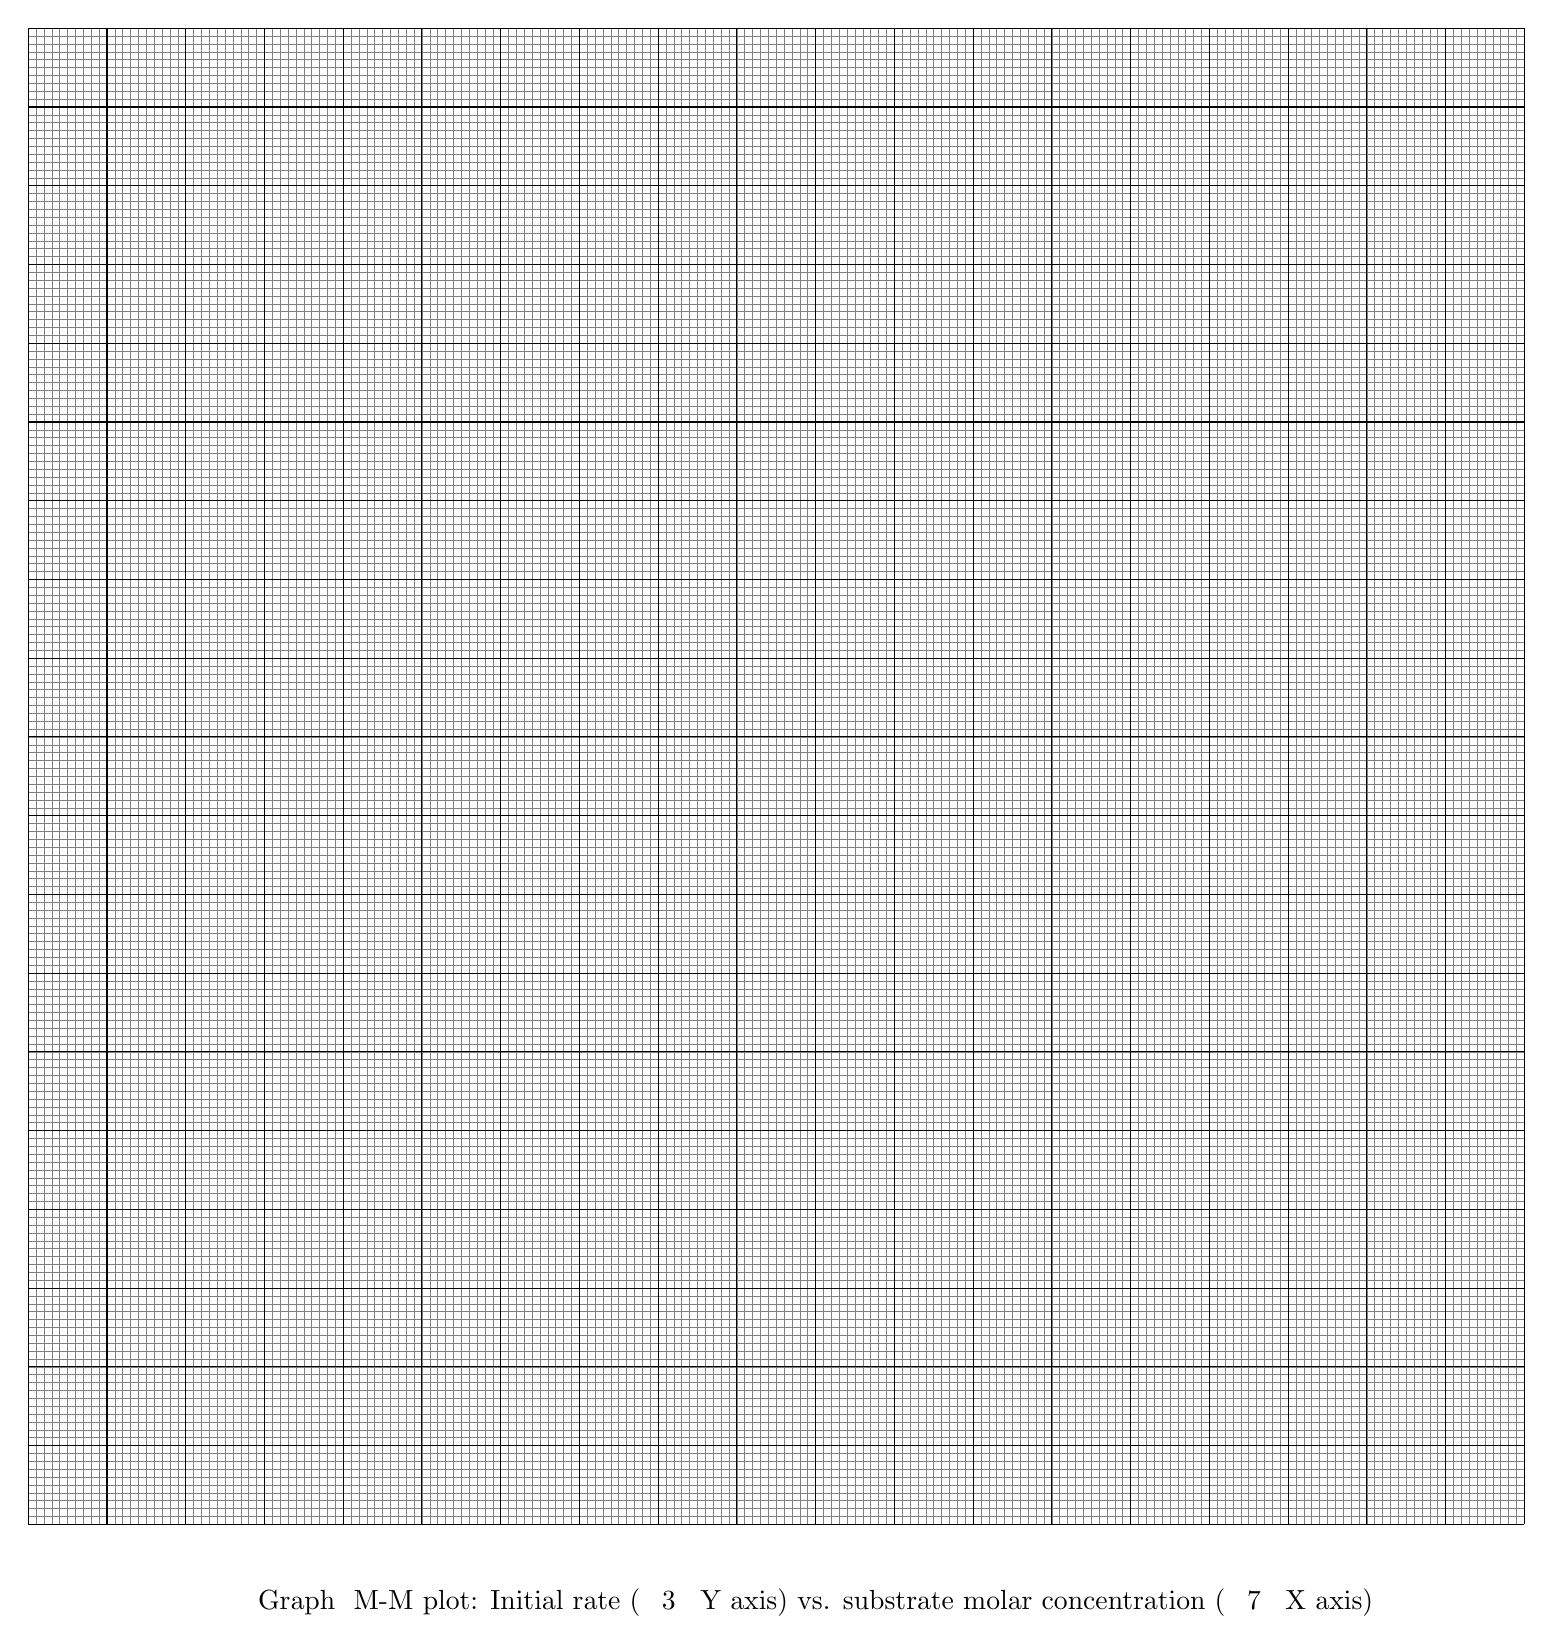
\begin{tikzpicture}
\begin{scope}[shift={(-15cm,-35cm)},rotate=0]
\draw[step=1mm,help lines] (0,0) grid (190mm,190mm);
\draw[step=10mm] (0,0) grid (190mm,190mm);
\end{scope}
\begin{scope}[shift={(-5cm,-36cm)},rotate=0]
\node[inner sep=0pt,rotate=0]   at (0,0) {Graph {\thegraphcounter} M-M plot:  Initial rate ( \:\:\mycircled{3} \: Y axis) vs. substrate molar concentration (  \:\:\mycircled{7} \: X axis)  };
\end{scope}
\end{tikzpicture}
\end{center}


\newpage
 \vspace{2cm}
\begin{center}
\stepcounter{graphcounter}   
 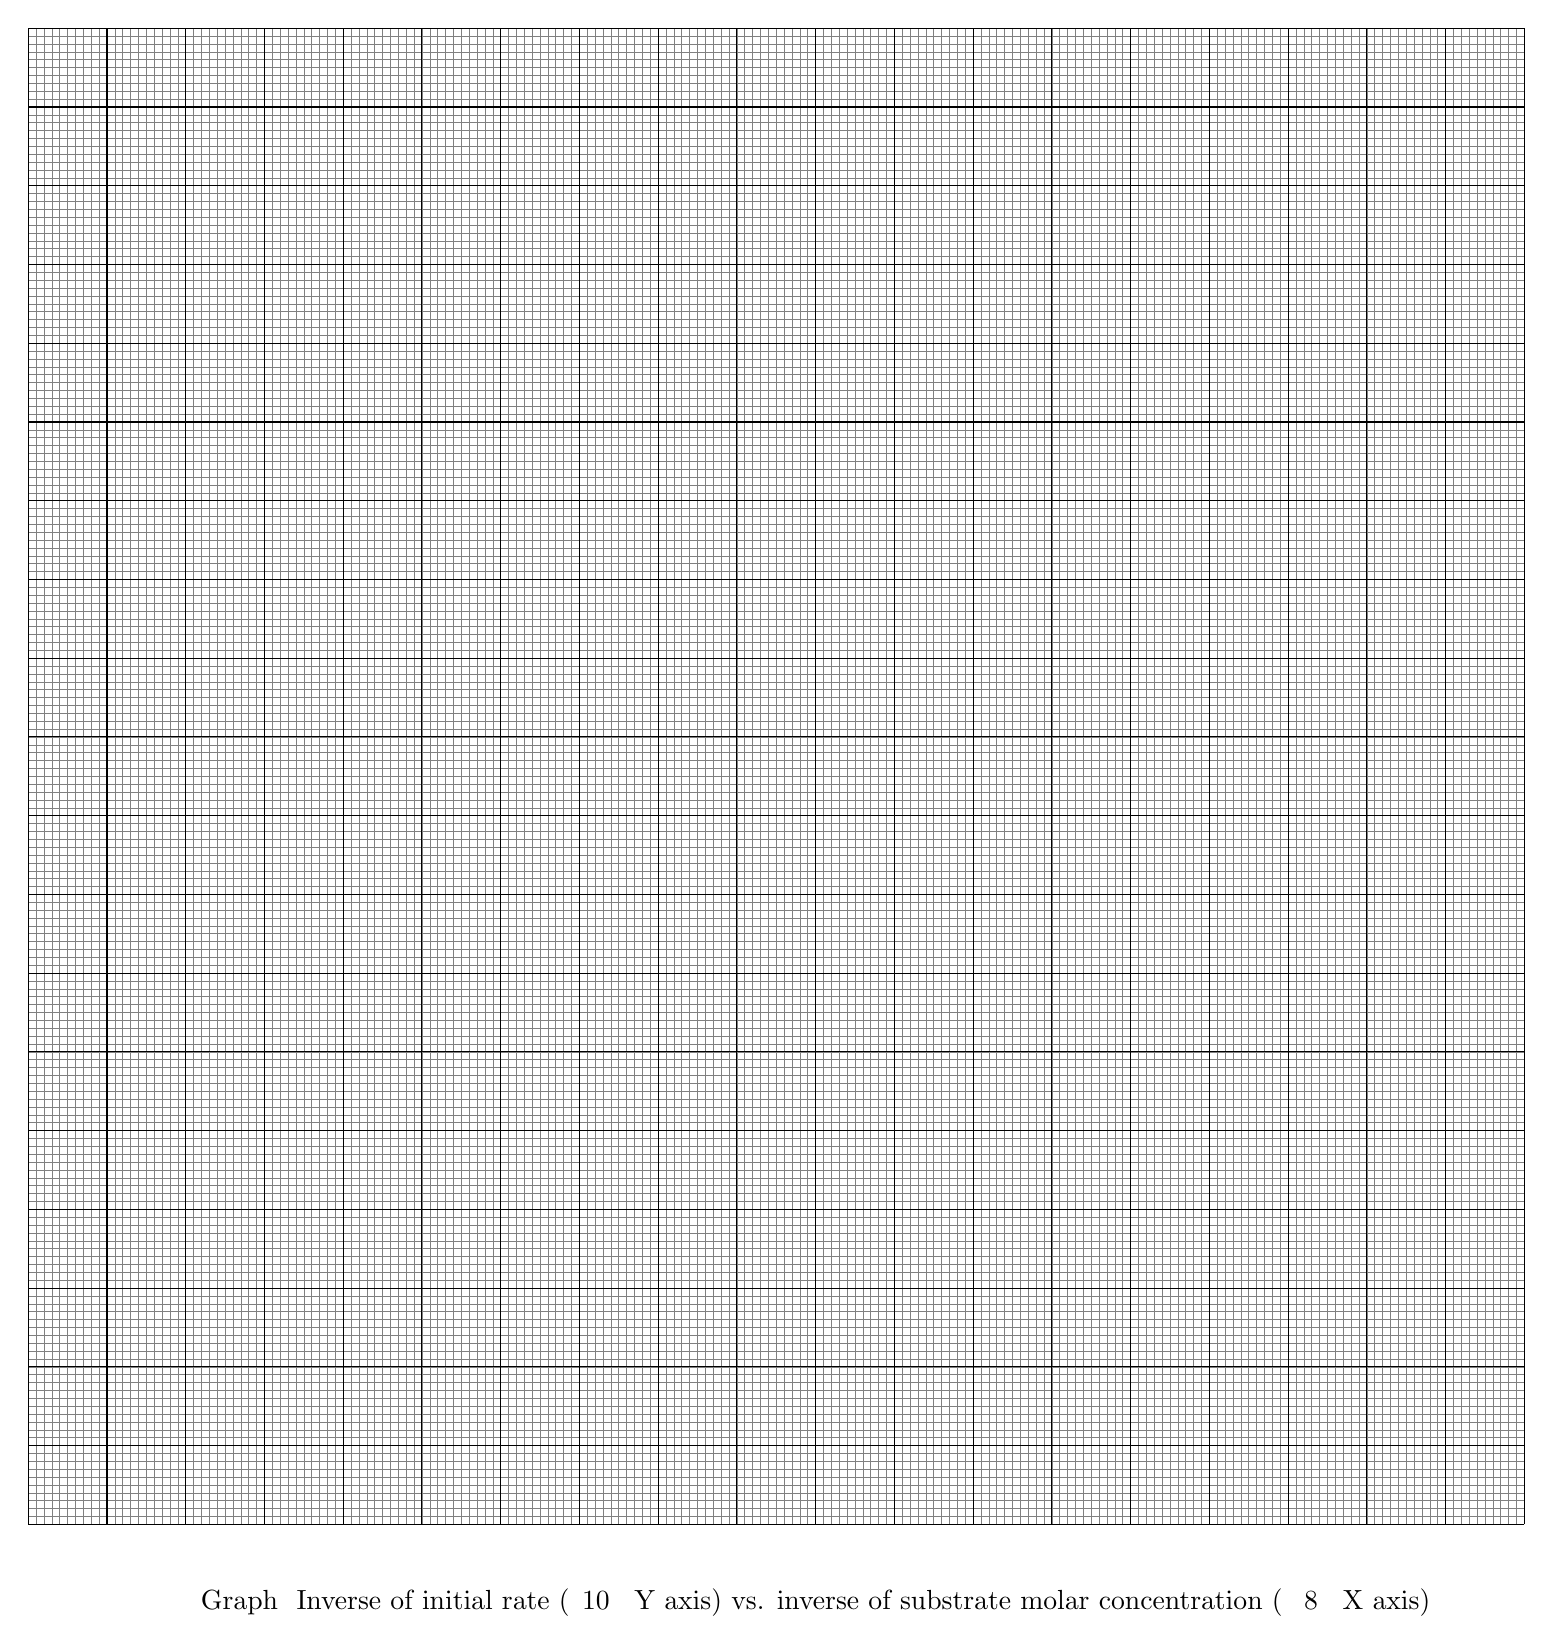
\begin{tikzpicture}
 \begin{scope}[shift={(-15cm,-35cm)},rotate=0]
 \draw[step=1mm,help lines] (0,0) grid (190mm,190mm);
 \draw[step=10mm] (0,0) grid (190mm,190mm);
  \end{scope}
 \begin{scope}[shift={(-5cm,-36cm)},rotate=0]
 \node[inner sep=0pt,rotate=0]   at (0,0) {Graph {\thegraphcounter} Inverse of initial rate (\:\:\mycircled{10} \: Y axis) vs.  inverse of substrate molar concentration ( \:\:\mycircled{8} \: X axis)  };
 \end{scope}
\end{tikzpicture}
\end{center}

   

%%%%%%%%%%%%HEADING
\newgeometry{right=5cm}\thispagestyle{sidebar}\sidebar{\vspace{1em}\vspace{1cm}\vfill\par\vspace*{1em}}\restoregeometry\clearpage \begin{multicols}{2}\begin{tcolorbox}[enhanced jigsaw,breakable,size=title,colback=mybrown!05,colframe=black,fonttitle=\bfseries,title=STUDENT INFO,pad at break=1mm, break at=15cm/0pt ]\vspace{0.2cm}\noindent Name:  \begin{Form}\TextField[name=NAME, width=4cm,height=0.5cm,multiline=false, borderstyle=U, bordercolor={black}]{} \end{Form}   \hspace{0.2cm}Date:  \begin{Form}\TextField[name=DATE, width=1.5cm,height=0.5cm,multiline=false, borderstyle=U, bordercolor={black}]{}\end{Form} \\\end{tcolorbox}\end{multicols}\hfill\vspace{0.2cm}\begin{center}{\large \bfseries Post-lab Questions \par\Huge
 \import{\chapterpath/}{title}
\\[5pt] \par}\vspace{0.2cm}\end{center}\par\noindent\uline{  \hfill \normalsize \hfill       }
%%%%%%%%%%%%HEADING
 \import{\chapterpath/}{postlab}

%\clearpage\mbox{}\clearpage

 \end{refsection}
\end{document}
